The problem at hand involves a time-dependent objective function, namely the fission gas release fraction throughout the course of a power ramp. Considering most surrogate methodologies, including the ones of interest in this thesis, are designed to handle single objective functions at a time, constructing a surrogate for an entire time series is problematic since a surrogate must be constructed at every time step. Such is especially the case when one does not know a priori whether or not a given time series will contain interesting features mid-cycle, such as jumps and peaks in the objective function. In addition, if pertinent experimental time series data is available and a calibration study is desired, a surrogate model for the entire time series will be necessary. Time dependency is not an issue if one is only interested in investigating, for example, beginning of life or end of life behavior.  
 
As with many of the great ideas in linear algebra, the premise of \ac{PCA} rests on a change of basis. \ac{PCA} attempts to represent some original data samples in terms of a set of basis vectors that reduce redundancy and noise in the data. To this end, consider a matrix $\textbf{X}$ of $n$ observations and $k$ variables where the $k$ variables have been rescaled by their respective mean, as shown in Eq. \ref{eq:dataMatrix}. Rescaling by the mean will ensure that the projected data will live around the centroid of the new basis vectors.
\begin{equation}
\label{eq:dataMatrix}
 \textbf{X} =
  \begin{pmatrix}
   \vline & \vline & \cdots & \vline \\ 
   X_{1} & X_{2} & \cdots & X_{k} \\
   \vline & \vline & \cdots & \vline 
  \end{pmatrix}
\end{equation} 
The problem \ac{PCA} solves is that of choosing a set of expansion coefficients $\lbrace p_{1j}\rbrace_{j=1}^k$ such that,
\begin{equation}
\label{eq:pcaExpCoeffs}
 \textbf{Y}_{1} = \textbf{p}_{1}^{T}\textbf{X}^{T} = p_{11}X_{1} + p_{12}X_{2} + \cdots + p_{1k}X_{k}
\end{equation}
captures the largest variance in the data set. In other words, $\textbf{Y}_{1}$ will point in the direction of largest variance. To bound the potential values of $\textbf{p}_{1}$ the condition $\| \textbf{p}_{1} \|_2 = 1$ is enforced. Since it is unlikely that $\textbf{Y}_{1}$ will capture all the variance in the data, \ac{PCA} goes on to find $\textbf{Y}_{2}, ..., \textbf{Y}_{k}$ such that all the variance in the data is accounted for. Each $\textbf{Y}_{j}$ is independent from the other $\textbf{Y}_{i\not= j}$ to make sure there is no redundancy in capturing variance. Each $\textbf{Y}_{j}$ is referred to as the $j$-principal component. In matrix form, the workings of \ac{PCA} result in,
\begin{equation}
\label{eq:pcaRotation}
 \textbf{Y} = \textbf{P}^T\textbf{X}^T.
\end{equation}
From Eq. \ref{eq:pcaRotation} it becomes clear that the operator $\textbf{P}$ consisting of $\lbrace p_{ij}\rbrace_{i,j=1}^k$ has the effect of rotating the data in $\textbf{X}$ onto an uncorrelated set of axis. 

While the desired effect of operator $\textbf{P}$ to produce output $\textbf{Y}$ has been described, the question of how to find the expansion coefficients comprising $\textbf{P}$ remains. As described in \cite{Shlens}, the coefficients can be shown to be the loadings of the eigenvectors of the covariance matrix for $\textbf{X}$. The columns of $\textbf{P}$ are the eigenvectors of the symmetric matrix, 
\begin{equation}
\label{eq:covarMatrixPCA}
  \begin{pmatrix}
   \sigma_{1,1} & \sigma_{1,2} & \cdots & \sigma_{1,k} \\
                  & \sigma_{2,2} & \cdots & \sigma_{2,k} \\
                  &                 & \ddots & \vdots        \\
                  &                 &          & \sigma_{k,k}
  \end{pmatrix}
\end{equation}
where $\sigma_{i,j}$ represents the covariance between random variables $X_i$ and $X_j$. The eigenvalues of the matrix in Eq. \ref{eq:covarMatrixPCA} represent the amount of variance covered by the respective eigenvector. Before being placed into $\textbf{P}$, the eigenvectors should be sorted in descending order with respect to eigenvalue. 

The utility of \ac{PCA} lays in the fact that for most data sets the variance can be projected onto $\mathcal{O}(1)$ eigenvectors. To reveal this property the sorted eigenvalues can be plotted consecutively. \ac{PCA} can be viewed as a tool for reducing the dimensionality of a data set by opting to keep only the first $r$-principal components since a majority of the variance can be projected onto these components. Indeed, if only $r$ eigenvectors are kept then the projected data can written as,
\begin{equation}
\label{eq:projectedDataPCA}
 \textbf{Y}_r = \textbf{P}_r^T \textbf{X}^T.
\end{equation} 
Using Eq. \ref{eq:projectedDataPCA} the reduced-variance version of the data in $\textbf{X}$ can be reconstructed as,
\begin{equation}
\label{eq:reconstructedDataPCA}
 \textbf{X}_*^T = \textbf{P}_r \textbf{Y}_r
\end{equation} 
where it's noted that the inverse of a matrix with orthonormal columns is its transpose. The reconstructed data in Eq. \ref{eq:reconstructedDataPCA} represents perturbations around a centroid; the data mean must be added back in to obtain physical values. Using \ac{PCA} to express a data set in terms of a more meaningful and truncated basis allows one to filter out noise and identify structure in the data. Such possibilities allow one to glean insights into the main contributors of a data set's variance \cite{Bisgaard}.  

To obtain insight into the contributors of variance in Bison fission gas release time series, \ac{PCA} is applied to the data shown in Fig. \ref{fig:fgrSimulations}. Each of the 100 time series shown in Fig. \ref{fig:fgrSimulations} is induced by a different set of \ac{SIFGRS} parameters. Consequently, the time-stepping required for convergence in Bison varies from one time series to another. To perform \ac{PCA} on the data, fission gas release fractions must be compared at identical times throughout the 100 different samples. Consequently every power ramp time series output by Bison is interpolated using cubic splines and then sampled at 150 evenly spaced points. The covariance matrix central to \ac{PCA} in this case contains covariances between all 150 time steps. The eigenvalues of the covariance matrix are depicted in Fig. \ref{fig:fgrEvals}.
\begin{figure}
\caption{\label{fig:fgrEvals}
Cummulative variance carried by successive eigenvalues in the \ac{PCA} covariance matrix.}
 \begin{center}
  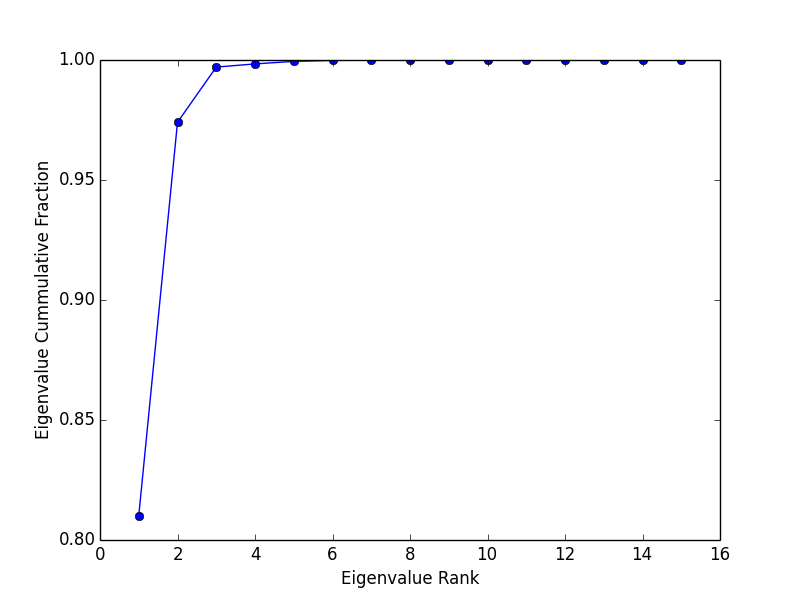
\includegraphics[scale=.75]{./Chapter4/fgr_evals.png}
 \end{center}
\end{figure}
As seen in Fig. \ref{fig:fgrEvals}, the three largest eigenvalues account for over 99\% of the variance. If the original time series data is rotated onto the corresponding three principal components using Eq. \ref{eq:projectedDataPCA}, each time series can be represented using only three expansion coefficients. Consequently, surrogates can be constructed for only the three expansion coefficients as a function of the \ac{SIFGRS} parameters. Instead of having to construct a surrogate at every time step, the principal component expansion coefficient surrogates act as a mapping to the entire time series.   

The three principal components corresponding to the three largest eigenvalues of the time series covariance matrix are plotted in Fig. \ref{fig:fgrEvecs}. The principal components enable insight into an underlying stochastic process by observing the magnitude of their coefficients \cite{Bisgaard}.  
\begin{figure}
\caption{\label{fig:fgrEvecs}
First three principal components of the time series covariance matrix.}
 \begin{center}
  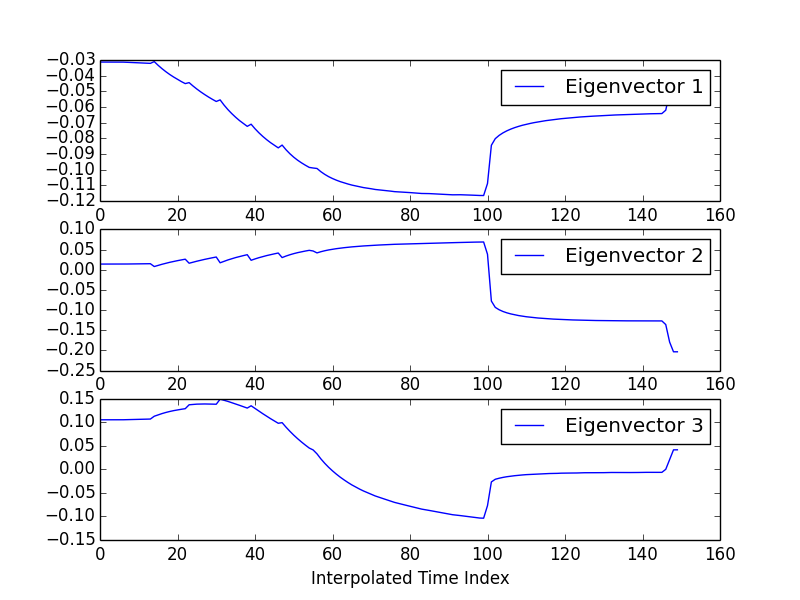
\includegraphics[scale=.75]{./Chapter4/fgr_evecs.png}
 \end{center}
\end{figure}
Each time index's magnitude in a principal component represents its influence on the component. From Fig. \ref{fig:fgrEvecs} it appears as though the first principal component is strongly influenced by the times in the middle of the power ramp, the second principal component is influenced by the times at the end of the power ramp and the third principal component is influenced most by the early stages of the power ramp. Further insights can be gleaned by plotting the principal components as time series and correlating the loadings with the \ac{LHS} values for the \ac{SIFGRS} parameters as in Fig. \ref{fig:principalCompTS}.     
\begin{figure}
\caption{\label{fig:principalCompTS}
Time series of the first principal component and correlations with \ac{SIFGRS} parameters.}
 \begin{center}
  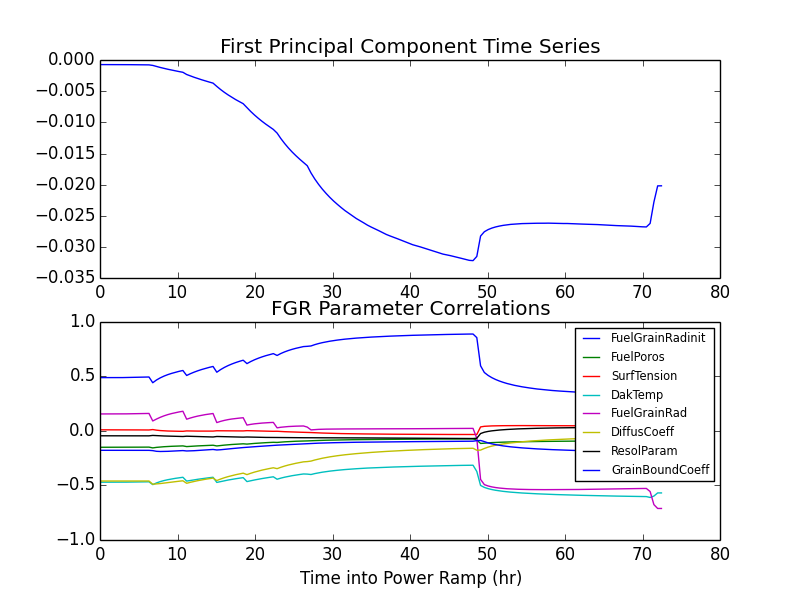
\includegraphics[scale=.75]{./Chapter4/firstPrincComp_FGR_Correlations.png}
 \end{center}
\end{figure}
The initial fuel grain radius appears to be the leading driver of the variance in the first principal component judging by its high correlation in the middle of the power ramp. Observe how in the late stages of the power ramp, the temperature and grain radius become primary contributors. 
